% xcolor is pulled in first by another package, so the table option has to be passed ahead
% of \documentclass or the second \usepackage is an option clash.
\PassOptionsToPackage{table}{xcolor}
\documentclass{article}
\usepackage{iclr2025_conference}
% NOT \usepackage{times}. Under this toolchain that package resolves to Latin Modern Roman with no bold
% and no italic face, so every \textbf and \emph in the paper renders at regular weight without an error.
% newtxtext supplies TeX Gyre Termes, which is Times, with all four faces.
\usepackage{newtxtext,newtxmath}
\usepackage{hyperref}
\usepackage{url}
\usepackage{graphicx}
\usepackage{booktabs}
\usepackage{amsmath}
\let\Bbbk\relax  % newtxmath already defines it; without this amssymb aborts the build
\usepackage{amssymb}
\usepackage{xcolor}
\usepackage{tcolorbox}
% Boxed, numbered, self-contained claims, after Liu et al. (NeurIPS 2025). A reader who takes only the
% boxes away should have the paper's argument; the surrounding prose is how each one was earned.
\definecolor{resbar}{HTML}{7B1E24}
\definecolor{resbg}{HTML}{F7EEEF}
\definecolor{qbar}{HTML}{1F3D5C}
\definecolor{qbg}{HTML}{EEF2F7}
\newtcolorbox{resultbox}[1]{colback=resbg, colframe=resbar, coltitle=white, fonttitle=\bfseries\small,
  title={#1}, boxrule=0.5pt, arc=1pt, left=5pt, right=5pt, top=3pt, bottom=3pt,
  boxsep=1pt, before skip=6pt, after skip=6pt}
\newtcolorbox{questionbox}[1]{colback=qbg, colframe=qbar, coltitle=white, fonttitle=\bfseries\small,
  title={#1}, boxrule=0.5pt, arc=1pt, left=5pt, right=5pt, top=3pt, bottom=3pt,
  boxsep=1pt, before skip=6pt, after skip=6pt}
\definecolor{sectbg}{HTML}{E9ECF2}   % banner rows: the grouping IS the result
\definecolor{medrow}{HTML}{FCF5EA}   % the two medical models
\definecolor{poscol}{HTML}{1B6E3C}
\definecolor{negcol}{HTML}{A8322C}

\title{Medical Vision-Language Models\\Do Not Use What They Encode}

\author{Anonymous}

\newcommand{\fig}[1]{Figure~\ref{fig:#1}}

\begin{document}
\maketitle

\begin{abstract}
A linear probe decodes a clinical finding from a layer of a medical vision-language model, and the finding
is said to be represented there. We present an alternative account of what such a score measures: it is
the sum of what any network of that shape provides, what training added, and nothing at all about whether
the model can use either. We state the account as a three-term decomposition and test it three ways on
five 7B-to-8B models, nine chest-radiograph findings and a second imaging modality.
First, against a floor given by the same probe on the \emph{same architecture with randomly initialised
weights}, training adds a median of 0.11 AUROC and the model's own zero-shot answer captures a median of
9\% of it; in 22 of 45 cells the answer is \emph{below} the untrained floor. The distribution is a
dichotomy rather than a gradient: two models reach $+121\%$ and $+83\%$ utilisation and three reach
$-61\%$, $-68\%$ and $-69\%$. Second, neither account that avoids ours survives: the best of four readouts
recovers a median of 7\% of the gap, and calibration cannot explain it because AUROC is invariant to
monotone rescaling. Third, we manufacture the phenomenon: a network that has never been trained decodes
the acquisition variable at 0.997 and reaches 0.54 to 0.79 AUROC on the nine findings, with a
\emph{positive} control-task selectivity higher than most trained models achieve.
The consequence for practice is direct. Probe AUROC spans 0.033 across the five models and behavioural
AUROC spans 0.179. Probing ranks these models as interchangeable and is wrong about three of them.
\end{abstract}

\section{Introduction}

Linear probing is the standard instrument for asking what a medical vision-language model has learned
\citep{alain2017understanding,belinkov2019analysis}. A classifier is fitted on the activations at some
layer, its held-out accuracy is reported, and the finding is said to be \emph{represented} there. The move
is routine enough that its two implicit claims are rarely written down.

\begin{enumerate}
\item \textbf{Attribution.} A high probe score is a fact about the model, so a model that probes better
      has learned more.
\item \textbf{Relevance.} A concept that is decodable is a concept the model is working with, so the layer
      where it decodes best is the place to intervene on it.
\end{enumerate}

Neither follows. \fig{teaser} shows why. On the same 1000 held-out radiographs, a probe fitted at the
connector reads the nine findings out of all five models we study to within 0.033 AUROC of one another.
Their own answers to the same questions differ by a factor of 5.3. The two models whose answers keep the
information are not the two medical ones, and nothing in the probe scores marks them out.

\textbf{A probe score is a sum of three things, and the field reports the sum.} A randomly initialised deep
network is a random feature map. A linear readout given eighteen thousand labels will find structure in it
whenever the label correlates with anything the image statistics carry, and in chest radiography the labels
correlate with a great deal: portable anteroposterior films are taken of sicker patients, so the view
position alone carries information about what is on the film. Whatever a probe extracts from an untrained
network of the same shape is not a fact about the trained model. What training adds on top of that is. And
whether the model can act on either is a third question a probe does not address.

\textbf{The controls that would separate them are almost never run.} In a survey of 135 medical
interpretability studies, a randomised control task \citep{hewitt2019designing} appears in \textbf{none},
a permutation null in 3 of 69 applicable records, and a randomly initialised encoder baseline in 5 of 121.
Section~\ref{sec:test3} shows that even the first of these, the strongest control the field has, does not
do the job: on an untrained network the control-task selectivity for cardiomegaly is $+0.17$, higher than
most trained models achieve.

\textbf{That a model may not use what it encodes is not a new suspicion.} It was raised on synthetic tasks
a decade into the probing literature \citep{ravichander2021probing} and has been reported this year for
text reasoning \citep{goel2026knowing} and for chart evidence \citep{kumar2026encoded}. What is missing is
a measurement: a quantity that says what \emph{share} of what training added the model reaches, on a scale
that makes models comparable. That requires the one control the field does not run, and it is what this
paper supplies.

\textbf{Contributions.}
\begin{itemize}
\item A three-term decomposition of a probe score and a normalised quantity, \emph{utilisation}, measuring
      what fraction of the information training added the model's own output pathway reaches
      (Section~\ref{sec:account}).
\item A measurement of all three terms on five models and nine findings. Median utilisation is 9\%; in 22
      of 45 cells the answer is below what a probe reads from an untrained network
      (Section~\ref{sec:test1}).
\item Elimination of the two accounts that do not require ours (Section~\ref{sec:test2}).
\item A demonstration that concept decodability can be manufactured without training at all
      (Section~\ref{sec:test3}).
\item The consequence for practice: probing ranks these five models as interchangeable and is wrong about
      three of them.
\end{itemize}

\begin{figure}[t]
\centering
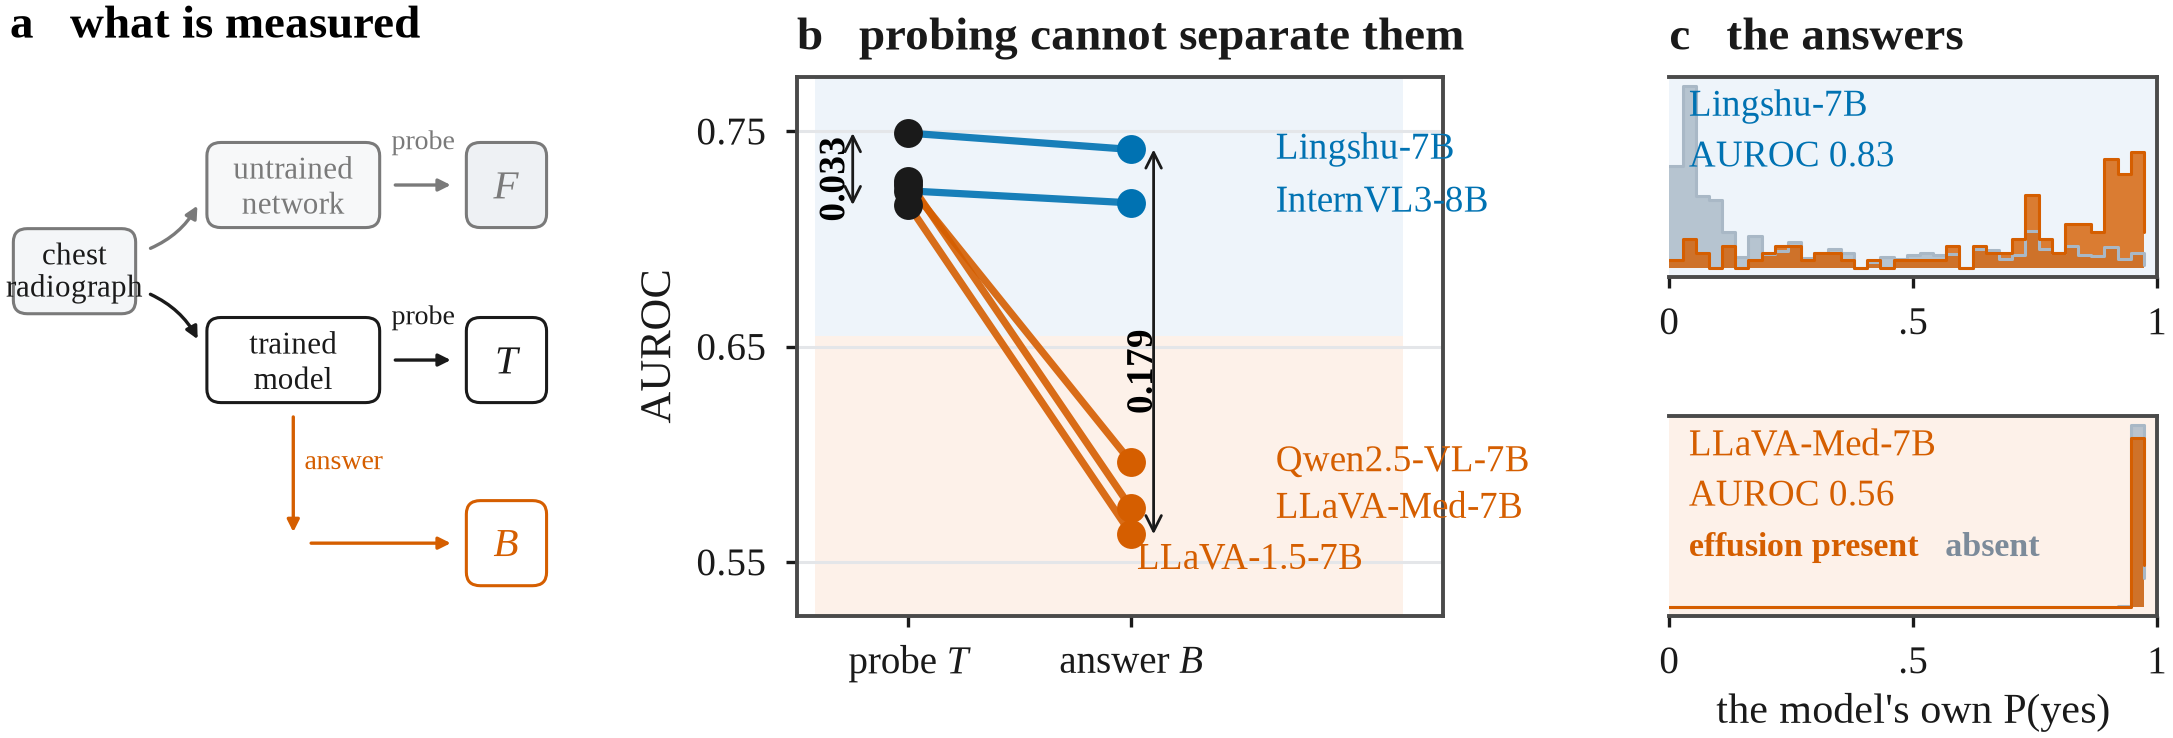
\includegraphics[width=\linewidth]{figures/fig_teaser.png}
\caption{\textbf{Five medical vision-language models that a probe cannot tell apart differ by 0.179 AUROC
in what they actually answer.} \textbf{(a)}: the three quantities, all measured on the same 1000 held-out
chest radiographs and the same labels. $F$ is a linear probe on an \emph{untrained} network of the same
architecture, $T$ the same probe on the trained model, and $B$ the AUROC of the model's own answer to ``is
there a pleural effusion?''. \textbf{(b)}: median over nine findings, one line per model, coloured by
whether the answer beats the untrained floor. Probe scores span 0.033; answers span 0.179. \textbf{(c)}:
the answer distributions behind two of those points, coloured by whether the finding is present.
LLaVA-Med-7B places 98.8\% of its answers outside $[0.05,0.95]$ with the classes superimposed at 0.967.}
\label{fig:teaser}
\end{figure}

\section{The Account, and How Each Term Is Measured}
\subsection{The account, and what it predicts}
\label{sec:account}

Let $\mathcal{V}$ be a family of linear readouts and $I_\mathcal{V}(X \to Y)$ the usable information about
label $Y$ extractable from representation $X$ \citep{xu2020theory}. Write

\begin{align*}
F &= \text{the probe's AUROC on an \emph{untrained} network of the same architecture,}\\
T &= \text{the probe's AUROC on the trained network,}\\
B &= \text{the AUROC of the model's own answer to ``is there a } Y \text{?''.}
\end{align*}

$F$ is neither zero nor chance. $T - F$ is what training added. $B$ is what the model does. The field
reports $T$, and $T$ alone licenses neither implicit claim: not attribution, because $F$ may account for
most of it, and not relevance, because nothing connects $T$ to $B$. We therefore report
\begin{equation}
\text{utilisation} \;=\; \frac{B - F}{T - F},
\label{eq:util}
\end{equation}
which is $0$ when the answer is no better than a probe on an untrained network, $1$ when the answer is as
good as any linear readout of the model's own activations, and negative when the answer is worse than the
untrained floor. Utilisation is invariant to the probe's supervision advantage, because that advantage is
present in $F$ and in $T$ alike and cancels.

The account makes three predictions, tested in turn below.

\begin{description}
\item[P1] Models with nearly identical $T$ will have widely different $B$, so probe scores will not rank
      models by what they do.
\item[P2] The gap $T - B$ will not close under better elicitation, because it is not a readout problem.
\item[P3] $F$ will be large and will exist before any training.
\end{description}

\label{sec:design}

\subsection{Models and data}

Five open-weight vision-language models at 7B to 8B parameters, chosen so that two \emph{architecture
matched} medical and general pairs are available: Lingshu-7B \citep{bai2025lingshu} against Qwen2.5-VL-7B
\citep{bai2025qwen25vl}, and LLaVA-Med-7B \citep{li2023llavamed} against LLaVA-1.5-7B
\citep{liu2024improved}, with InternVL3-8B \citep{zhu2025internvl3} as a fifth. Within a pair the two
models share every architectural constant, down to hidden width, layer count, connector type and the
number of visual tokens. They therefore share an untrained floor exactly, and any difference in
utilisation between them is attributable to training and to nothing else. We are aware of no other pair of
public medical and general vision-language models for which this holds.

\textbf{Chest radiographs.} NIH ChestX-ray14 \citep{wang2017chestxray}, 26{,}229 frontal radiographs
carrying nine findings mined from radiology reports. The split is by patient rather than by image, which
matters because the dataset contains several studies per patient and an image-level split leaks a
patient's anatomy across the boundary. A SHA-256 hash of the patient identifier, with a fixed salt,
assigns each patient to train, validation or test, and we assert at build time that no patient appears on
both sides of any split. This yields 18{,}212 training rows and 5{,}343 test rows drawn from 1{,}659 test
patients. Nine findings are used throughout: effusion, cardiomegaly, pneumothorax, atelectasis,
consolidation, oedema, infiltration, mass and nodule.

\textbf{Dermoscopy.} The second modality is the ISIC archive \citep{codella2019skin}: 12{,}012 dermoscopic
images over 4{,}109 patients with six diagnoses at 300 or more examples, filtered from the full index of
553{,}019 records and split by the identical hash procedure with the identical assertion
(Appendix~\ref{app:mod}). The design mirrors the radiograph design, with anatomic site standing in for
view position as the acquisition nuisance.

\subsection{How each of the three terms is computed}

All three terms are AUROCs against the same labels on the same 1000 held-out radiographs, drawn once with
a fixed seed and reused for every model and every term. Nothing is selected on the test labels.

\textbf{$T$, the probe on the trained model.} A single forward pass per image caches the activation at
every locus, pooled by a mean over that locus's positions; logistic regression is fitted on the training
rows and scored on the held-out rows. Capacity is fixed across loci and models by three choices made once:
one decoder class, one regularisation strength, and a random projection of every locus to a common width
of 512, so a wider representation cannot win on width alone.

\textbf{The locus is the connector, and it was fixed before any result was seen.} A probe may be fitted at
any of 64 to 72 loci and the best one reported, while the model's answer has no such choice; comparing a
selected statistic against an unselected one inflates the gap. The connector is also upstream of the
language model, so its activation does not depend on which question is asked. We report the maximum over
loci beside it only as an explicitly labelled upper bound, and every claim in the paper rests on the fixed
locus. The choice does not matter: over the 38 to 44 prompt-independent loci of each model, the sign of
utilisation is the same at every one, 192 model-by-locus points without a single change
(Appendix~\ref{app:depth}).

\textbf{$F$, the untrained floor.} The same architecture is instantiated from its configuration with
freshly initialised weights, and activations are extracted at the same loci with the same pooling, the
same prompt and the same batch structure. The probe is then fitted with the identical procedure. $F$ is
therefore what a linear map plus 18{,}212 labels extracts from a network of that shape with no training at
all. Because a floor depends only on the architecture and the seed, Lingshu and Qwen2.5-VL share one
untrained model and LLaVA-Med and LLaVA-1.5 share the other.

\textbf{$B$, the model's own answer.} The model is asked ``Is there a $c$ in this chest radiograph? Answer
yes or no.'' and we read $\log P(\text{yes}) - \log P(\text{no})$ at the answer position, taking the
maximum over the single-token surface forms of each word. No threshold is applied at any point, so $B$
measures the ranking the model induces over images rather than its decision rule. This distinction is what
makes the calibration objection in Section~\ref{sec:test2} closable by construction.

\subsection{The validity battery every probe number carries}

Every probe number reported here carries four controls: a permutation null, a randomised control task
\citep{hewitt2019designing} whose input type is the cross of the acquisition variable, sex and age decade,
nuisance probes for the acquisition variable and sex at the same locus from the same features, and the
untrained floor. Appendix~\ref{app:battery} gives the construction of each, including why a control task
over two input types is degenerate and what its failure looks like. Appendix~\ref{app:prompt} records
which loci depend on the prompt: changing the question moves answer-position activations by 6\% to 34\% in
relative norm and visual, connector and vision-tower activations by exactly $0.000000$, so answer-position
loci are used only for the finding whose question was cached and every number in this paper comes from a
prompt-independent locus.

\section{Results}

\subsection{A probe score does not rank models by what they do}
\label{sec:test1}

\textbf{Result.} Table~\ref{tab:main} gives the per-model summary and \fig{main} every cell. Over 45 cells the median
utilisation is 9\%, and in 22 of 45 the answer is below the
untrained floor. The distribution is bimodal rather than graded (\fig{main}): Lingshu-7B reaches a median
utilisation of $+121\%$ and InternVL3-8B $+83\%$, with no cell below the floor in either; Qwen2.5-VL-7B,
LLaVA-Med-7B and LLaVA-1.5-7B reach $-61\%$, $-68\%$ and $-69\%$, below the floor on 7, 8 and 7 of nine
findings.


% Grouped by the result rather than by name: the dichotomy is the finding, so it is the table's spine.
% Superscripts on F mark the two architecture-matched pairs, which share a floor exactly.
% The small rank in T and in B is the paper's first claim made visible: the two orderings cross.
\begin{table}[t]
\centering
\caption{\textbf{The probe ranking and the behavioural ranking are different rankings.} Medians over the
nine findings, at the connector. $F$ is the same probe on the \emph{same architecture with randomly
initialised weights}, $T$ the probe on the trained model, $B$ the AUROC of the model's own
$P(\mathrm{yes})$, and $U=(B-F)/(T-F)$. The small numeral after $T$ and $B$ is that model's rank on the
column: LLaVA-Med-7B is second by probe and fourth by answer, InternVL3-8B fourth by probe and second by
answer. Models sharing a dagger are the same architecture and share a floor exactly.
Medical models are tinted. The last row is the half-width of a 95\% bootstrap
interval on a single probe estimate, 2000 resamples over the same 1000 images. Measured against that
uncertainty, the whole spread of $T$ across the five models is one half-width and the spread of $B$ is
5.4 of them.}
\label{tab:main}
\small
\setlength{\tabcolsep}{5.5pt}
\renewcommand{\arraystretch}{1.12}
\begin{tabular}{@{}l@{\hskip 13pt}ccc@{\hskip 13pt}cc@{\hskip 13pt}c@{\hskip 10pt}c@{}}
\toprule
 & \multicolumn{3}{c}{\textit{what a probe sees}} & \multicolumn{2}{c}{\textit{what the model does}}
 & \multicolumn{2}{c}{\textit{controls}} \\
\cmidrule(lr){2-4}\cmidrule(lr){5-6}\cmidrule(lr){7-8}
Model & $F$ & $T$ & $T{-}F$ & $B$ & $U$ & below $F$ & $\Delta$\,elicit \\
\midrule
\rowcolor{sectbg}\multicolumn{8}{l}{\textit{\,Utilisation positive: the answer reaches what training added}} \\
\rowcolor{medrow}
Lingshu-7B {\scriptsize(medical)}   & 0.659$^{\dagger}$  & 0.749\,{\scriptsize(1)} & $+$0.118 & 0.742\,{\scriptsize(1)} & \textcolor{poscol}{$+$121\%} & 0\,/\,9 & $+$0.000 \\
InternVL3-8B {\scriptsize(general)} & 0.552              & 0.722\,{\scriptsize(4)} & $+$0.162 & 0.717\,{\scriptsize(2)} & \textcolor{poscol}{$+$83\%}  & 0\,/\,9 & $+$0.015 \\
\rowcolor{sectbg}\multicolumn{8}{l}{\textit{\,Utilisation negative: the answer falls below a probe on untrained weights}} \\
Qwen2.5-VL-7B {\scriptsize(general)} & 0.659$^{\dagger}$  & 0.725\,{\scriptsize(3)} & $+$0.092 & 0.596\,{\scriptsize(3)} & \textcolor{negcol}{$-$61\%} & 7\,/\,9 & $+$0.016 \\
\rowcolor{medrow}
LLaVA-Med-7B {\scriptsize(medical)}  & 0.647$^{\ddagger}$ & 0.727\,{\scriptsize(2)} & $+$0.090 & 0.575\,{\scriptsize(4)} & \textcolor{negcol}{$-$68\%} & 8\,/\,9 & $+$0.000 \\
LLaVA-1.5-7B {\scriptsize(general)}  & 0.647$^{\ddagger}$ & 0.716\,{\scriptsize(5)} & $+$0.101 & 0.563\,{\scriptsize(5)} & \textcolor{negcol}{$-$69\%} & 7\,/\,9 & $+$0.034 \\
\midrule
\multicolumn{1}{l}{\textit{spread across the five}} & 0.107 & \textbf{0.033} & 0.072 & \textbf{0.179} & 190 pts & --- & 0.034 \\
\multicolumn{1}{l}{\textit{95\% interval, one estimate}} & & $\pm$0.033 & & & & & \\
\bottomrule
\end{tabular}
\end{table}

Lingshu exceeds 100\%, meaning its answer separates the labels better than any linear readout of its own
connector. That is not an anomaly: the remaining twenty-eight layers are not a linear map, and a model
whose later computation is doing useful work should exceed a linear readout of an intermediate layer. It
does mean utilisation is a comparison rather than a fraction, and we say so in the limitations.

\textbf{The shape of the distribution matters as much as its median.} Nothing lies between $+83\%$ and
$-61\%$, and within a model the nine findings agree, so the dichotomy is a property of models rather than
of particular findings. Whatever produces high utilisation is something a model either has or does not.

\textbf{P1 confirmed.} Median probe AUROC spans 0.033 across the five models, which is less than the
half-width of a
95\% bootstrap interval on any one of them, which is 0.033 as well. Any two of the five probe estimates
have overlapping intervals, so the instrument does not resolve these models at all. Median behavioural AUROC
spans 0.179, a factor of 5.3 (\fig{main}b). A study reporting only $T$ would call these models equivalent.

\textbf{The matched pair isolates training.} Lingshu and Qwen2.5-VL are the same architecture and share the
same untrained floor, so every difference between them is what training did. They differ by 183 points of
utilisation while their probe AUROCs agree to within 0.01 on six of nine findings (\fig{main}c). The LLaVA
pair differs by half a point, so medical pretraining is not the operative variable. That contrast also
rules out an instrument failure: a measure returning a negative number for every model would be suspect,
and this one returns $+121\%$ for one and $-69\%$ for another.

\textbf{The extreme case.} LLaVA-Med answers yes to all nine findings on all 1000 radiographs. For pleural
effusion its $P(\mathrm{yes})$ has mean 0.967 and standard deviation 0.006. A probe reads effusion from its
activations at 0.79. Every one of those probe numbers is correct, and none tells you the model will say yes
to whatever it is shown.

\begin{resultbox}{Result 1: a probe score does not rank models by what they do}
Against a floor given by the same probe on the same architecture with random weights, the model's own
answer captures a median of 9\% of what training added and falls \emph{below} the floor in 22 of 45 cells,
in a dichotomy ($+121\%$, $+83\%$ against $-61\%$, $-68\%$, $-69\%$) with nothing between. Probe scores
span 0.033 across the five, the half-width of one bootstrap interval; their answers span 0.179.
\end{resultbox}

\begin{figure}[t]
\centering
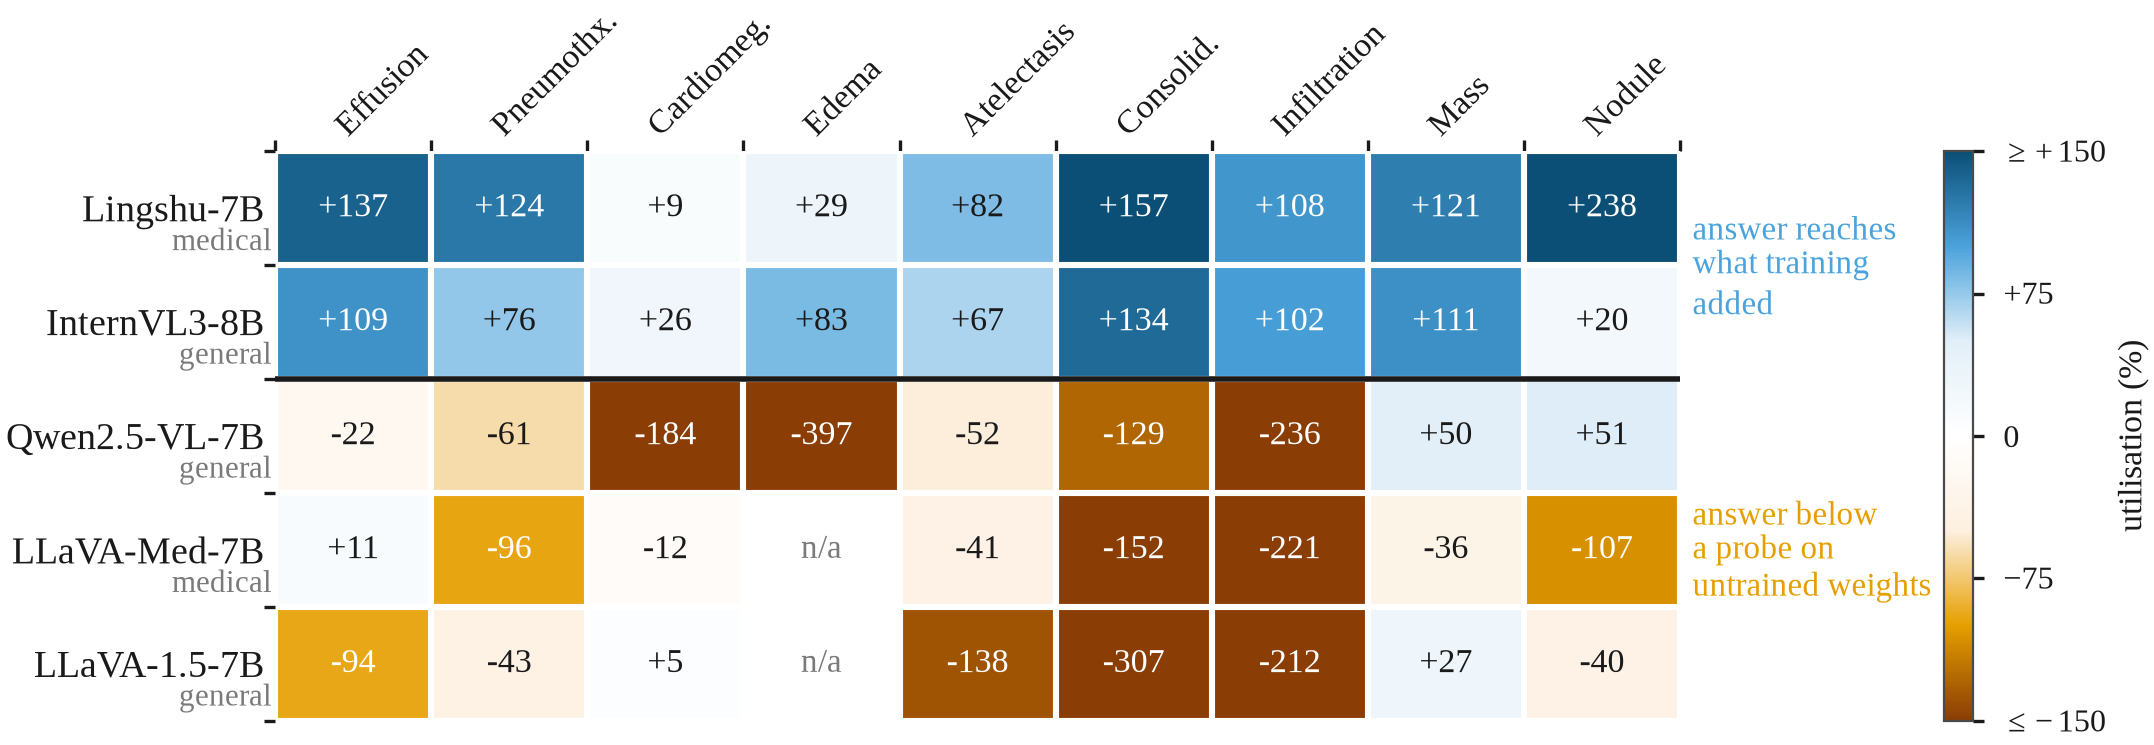
\includegraphics[width=\linewidth]{figures/fig_heat.png}
\caption{\textbf{All 45 cells, and nothing between the two groups.} Utilisation $(B-F)/(T-F)$ for every
model and finding, on a diverging scale pinned to white at zero, where zero means the model's answer
separates the labels exactly as well as a probe on untrained weights of the same architecture. The scale
is clipped at $\pm150\%$; three cells run past $-200$. Two models are positive on 9 of 9 findings and
three are negative on 7, 8 and 7 of 9, with no model between $+83\%$ and $-61\%$. Edema is undefined for
the two LLaVA models because training adds nothing there ($T \le F$), which the ratio cannot express.}
\label{fig:main}
\end{figure}


\subsection{The gap is not a readout problem}
\label{sec:test2}

\textbf{Better elicitation.} Four readouts on identical images: the original yes-or-no question, a
different phrasing, the log-probability of the full statement ``Yes, there is a $c$.'' against ``No, there
is no $c$.'', and a negation-symmetrised score that cancels a fixed response bias. Twenty
model-by-finding cells. The best of the four closes a median of 7\% of the gap, moving it from 0.177 to
0.170; the largest gain in any cell is 0.075; in 7 of 20 cells the original question is already the best
(\fig{controls}). On Lingshu the best gain is exactly 0.000 on all four findings, because there is no gap
to close. \textbf{P2 confirmed} (\fig{controls}).

The four readouts are not arbitrary. The second varies surface form while holding content fixed, which
isolates phrasing. The third replaces a single-token yes-or-no decision with the log-probability of a
complete clinical statement, which removes any dependence on how the model tokenises a bare ``yes''. The
fourth asks the negated question and subtracts, which cancels any response bias that is constant across
the two forms. Between them they cover the three mechanisms by which a readout, rather than a
representation, could be responsible for the gap.

A null result here is only informative if the readouts could have helped, and on some cells they do. The
negation-symmetrised score gains 0.075 on InternVL3 and pneumothorax and 0.043 on LLaVA-1.5 and oedema.
The method works; there is simply not much for it to recover.

\textbf{Calibration.} AUROC is invariant to any strictly monotone transform of the score, so a constant
tendency to answer yes cannot lower it \citep{zhao2021calibrate}. LLaVA-Med's yes rate is a statement about
its threshold; its AUROC is a statement about its ranking, and no recalibration, per-model or per-image
with a content-free input, changes a ranking. This account is closed by construction rather than by
experiment, which is why we spend no measurement on it.

\begin{resultbox}{Result 2: the gap is not a readout problem, and cannot be a calibration one}
The best of four readouts closes a median of 7\% of the gap over twenty cells, and in 7 of 20 the original
question is already the best. Calibration is closed by construction rather than by experiment: AUROC is
invariant to any strictly monotone transform of the score.
\end{resultbox}

\subsection{Concept decodability can be manufactured without training}
\label{sec:test3}

If $F$ is what any network of that shape provides, a network that has never been trained should already
produce respectable concept decodability.

\textbf{An untrained network decodes the acquisition variable.} A randomly initialised LLaVA-Med reads view
position at AUROC 0.9974 and a randomly initialised Qwen2.5-VL architecture at 0.996, against 0.9992 for
the trained LLaVA-Med. \textbf{The floor it produces is large.} Across the nine findings an untrained
network reaches 0.540 to 0.793 AUROC. Oedema reads at 0.793 from a network that was never trained, and
training adds 0.039 on top of it.

\textbf{A caution we state rather than hide.} The obvious account of that spread is that a finding's floor
follows its label's correlation with view position, and the association is in the right direction:
Pearson $r = +0.65$ across the nine findings. With nine points it is not significant
($p = 0.06$; Spearman $\rho = 0.50$, $p = 0.17$), and removing oedema leaves $r = 0.42$. The same analysis
on the Qwen architecture gives $r = +0.55$, $p = 0.13$. We report this as an association and not as
evidence. \textbf{P3 rests on the level of the floor, not on its explanation.}

\textbf{The strongest control the field has does not close this.} A randomised control task
\citep{hewitt2019designing} removes the contribution a probe's capacity makes. On an untrained
Qwen-architecture network it does not remove this one: selectivity is $+0.174$ for cardiomegaly and
$+0.219$ for oedema, higher than most trained models achieve on the same findings. Cardiomegaly is the size
of a shape, a low-level image statistic, and does not correlate with view position ($r = -0.020$), so the
control task does not absorb it. Only the untrained-network floor does.


\subsection{The floor is a property of the data, not of the network}
\label{sec:floor}

The account says $F$ is what \emph{any} network of that shape provides, which is a claim about the images
rather than about the weights. It can be wrong, and it makes a prediction that can refute it. Our five
models are built on three architecturally unrelated untrained networks, sharing no width, no depth, no
connector and no weights. If $F$ is the image statistics read through an arbitrary map, those three must
agree about \emph{which} findings are decodable. If $F$ is an accident of one random initialisation, they
should agree no better than chance.

\textbf{They agree.} The mean pairwise Spearman correlation between the rankings the three untrained
architectures induce over the nine findings is $\rho = +0.81$ (pairwise $+0.93$, $+0.85$, $+0.65$).
Against 20{,}000 random rankings the null has mean $-0.00$ and a 95th percentile of $+0.37$, giving
$p = 0.0001$ (\fig{floor}).

\textbf{And what training adds is unrelated to what the answer reaches.} Within a model, across the nine
findings, the partial correlation between the trained probe and the answer, holding the floor fixed, is
$+0.15$ with a 95\% interval of $[-0.33, +0.62]$. The raw correlation between $T-F$ and $B-F$ is $+0.28$,
but $T-F$ and $B-F$ share the term $-F$, which induces a positive correlation between them whatever the
data; the partial correlation removes it. We report the corrected number.

\begin{resultbox}{Result 3: the floor is a fact about the images, and what training adds is not what the answer reaches}
Three unrelated untrained architectures rank the nine findings alike, $\rho = +0.81$ against a permutation
null of zero, $p = 0.0001$: $F$ is what the image statistics make available through an arbitrary map, not
an artefact of one initialisation. Holding it fixed, what training adds carries no information about what
the answer reaches, $r = +0.15$, $[-0.33, +0.62]$.
\end{resultbox}

\begin{figure}[t]
\centering
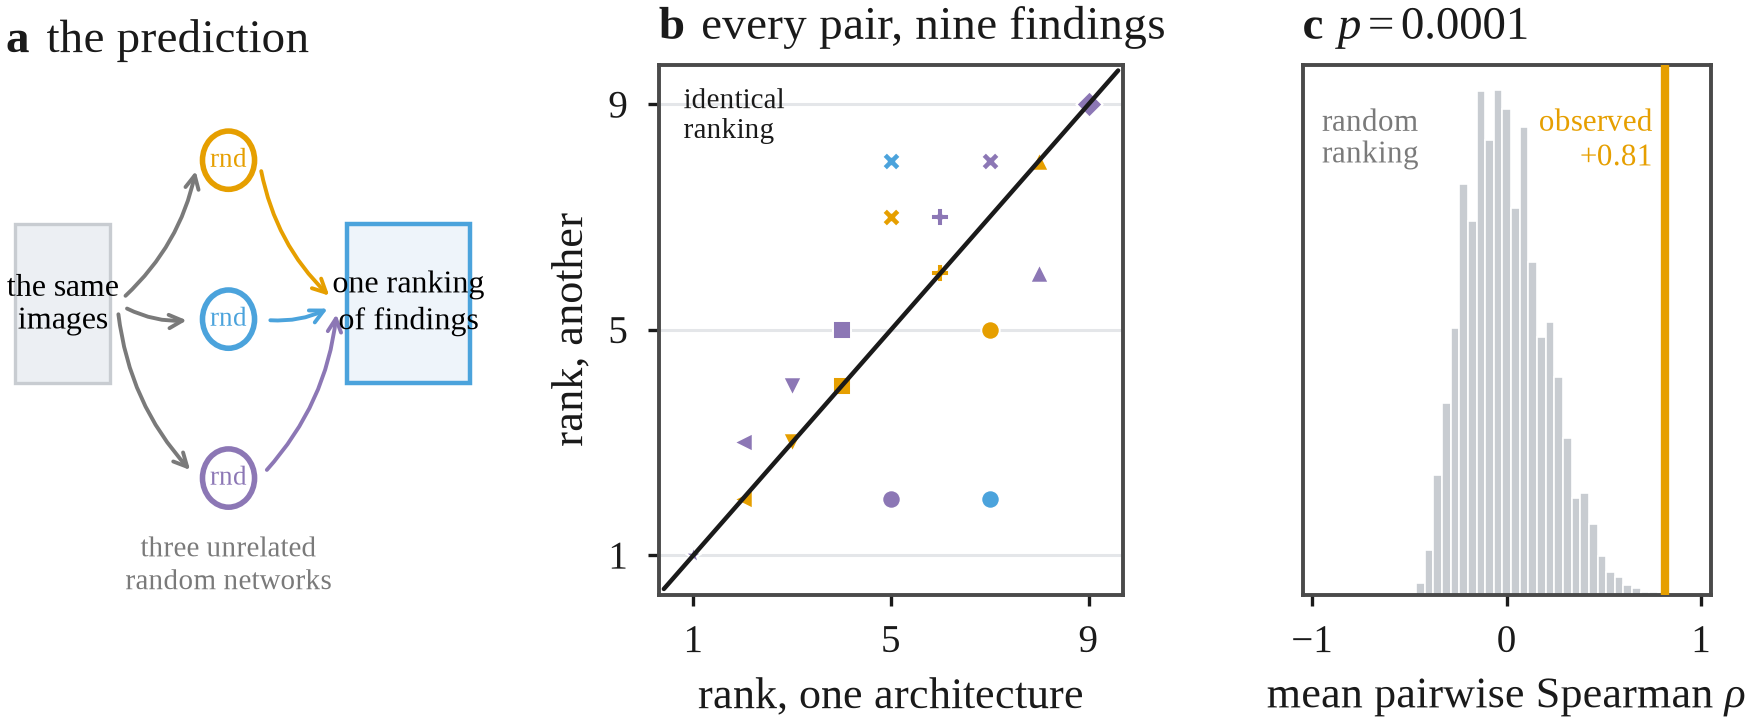
\includegraphics[width=\linewidth]{figures/fig_floor.png}
\caption{\textbf{Three unrelated random networks agree about which findings are decodable.}
\textbf{(a)}: the prediction. If the floor is the image statistics read through an arbitrary map, the
ranking it induces over findings is a fact about the images and must be common to all three untrained
architectures. \textbf{(b)}: the test. Every pair of architectures, nine findings, rank against rank,
with the identity line the prediction; colour is the architecture and shape the finding. \textbf{(c)}:
the null. Mean pairwise Spearman over 20{,}000 random rankings against the observed $+0.81$.}
\label{fig:floor}
\end{figure}

\subsection{Where the probe direction points}
\label{sec:direction}

Sections \ref{sec:test1} to \ref{sec:test3} concern the first implicit claim, attribution. This section
concerns the second, relevance: if a finding decodes best at some locus, is the probe normal there the
direction along which the model represents it?

\textbf{The probe normal is not intervention-optimal.}

We add $\alpha \lVert h_t \rVert v_{\text{probe}}$ to the residual stream token by token at 12 loci per
model, with $\alpha$ a fraction of that token's own activation norm so that a given $\alpha$ is the same
relative perturbation everywhere. The control battery at each locus is 16 random unit directions, 4 probe
normals for unrelated findings and one coordinate-permuted sham, all applied at the same magnitudes on
held-out images.

\textbf{The probe normal moves the model's answer no more than a random vector of the same norm in 26 of
50 cells} (\fig{dir}b). The cloud straddles the identity line: adding the direction a probe says encodes
effusion does about as much to the model's answer as adding an arbitrary direction of the same length,
and which of the two does more is close to a coin toss.

One locus in the sweep is a structural zero and is included deliberately. Perturbing the visual positions
at the final decoder layer cannot reach the answer position, because no attention layer follows. Measured
on Lingshu-7B with a random unit direction at full magnitude, that locus moves the logits by exactly
$0.00000$ while the layer below moves them by 1.03. A non-zero reading there would indict the measurement
rather than describe the model, and the sweep reads exactly zero.

\textbf{A direction fitted on behaviour is no more aligned with the probe normal than chance.}

Alongside $v_{\text{probe}}$ we fit a second unit vector by gradient descent on behaviour alone: it
maximises the change in $P(\mathrm{yes})$ for one finding's question minus three times the mean absolute
change for two other findings, and it never sees a label. The specificity penalty is load-bearing, since
without it the optimiser converges on a generic ``answer yes'' direction with a target-to-control ratio of
1.9 against 11.3. The fitted direction's cosine with the probe normal is 0.0135, against 0.0091 for a
random vector, which in 3584 dimensions is the floor: the direction that best \emph{writes} a finding into
the answer is no more aligned with the one that best \emph{reads} it than chance predicts.

\textbf{Planted ground truth.}

The comparisons above are between candidate directions with no ground truth. To obtain one we plant a
smooth opacity of known intensity at an anatomically plausible site in radiographs the model reads as
normal, and record the activation displacement it causes. That displacement is the direction the
representation travels when the finding is genuinely added to the input.

The lesion is a controlled perturbation and not a clinically realistic one, so it earns its use only by
passing a gate: the dose response must be monotone and must separate from a control blob of identical
intensity placed outside the thorax. It passes in 9 of 15 cells, with site ratios from 4.4 to 754; the six
failures are three cells whose baseline answer is pinned above 0.92 and three whose dose response is not
monotone. On the passing cells the mean absolute cosine with the true displacement is \textbf{0.0041 for
the probe normal, 0.0126 for a random vector and 0.0442 for the fitted direction} (\fig{dir}a). The probe
normal is three times \emph{less} aligned with the displacement the representation actually undergoes than
an arbitrary direction is, and beats a random vector in only 46 of 270 locus-by-dose rows.


\begin{resultbox}{Result 4: the direction a probe defines is not the direction the model uses}
Against a planted lesion, the probe normal's alignment with the displacement the representation actually
undergoes is flat at $0.004$ at every dose, below the $0.013$ of an arbitrary direction, while a direction
fitted on behaviour climbs to $0.044$. It moves the answer less than a random vector in 26 of 50 cells.
\end{resultbox}

\subsection{A second modality decides what generalises}

The identical battery on 12{,}012 ISIC dermoscopy images \citep{codella2019skin} over 4{,}109 patients,
with anatomic site standing in for view position. On chest radiographs the acquisition variable outranks
every clinical finding in all five models; on dermoscopy it does so in one of five
(Appendix~\ref{app:mod}), and median selectivity is $+0.050$ against $+0.308$. The structural results
reproduce; the quantitative one does not, so acquisition dominance is a chest-radiograph result and not a
property of medical vision-language models. Part of the difference is label quality and framing rather than
representation: NIH labels are mined from reports, ISIC diagnoses are largely biopsy-confirmed, and
dermoscopy is lesion-centred.

\section{Related Work}

\textbf{Probing and its controls.} Linear probes ask what a representation makes linearly available
\citep{alain2017understanding,belinkov2019analysis}. \citet{hewitt2019designing} showed that probe
accuracy confounds what the representation carries with what the probe can fit, and proposed selectivity
as the remedy; selectivity controls the probe's \emph{capacity}, not what the \emph{input statistics}
provide, and Section~\ref{sec:test3} exhibits an untrained network scoring $+0.17$ on it.
\citet{ravichander2021probing} make the prior version of our argument on synthetic tasks where a property
is provably irrelevant: they establish that the failure mode exists, we measure its size on deployed
models. \citet{heap2025automated} report the same hazard for a different instrument, sparse autoencoders
scoring a randomly initialised transformer as interpretably as a trained one.

\textbf{Usable information.} \citet{xu2020theory} define predictive $\mathcal{V}$-information, the
information about $Y$ extractable from $X$ by a bounded family $\mathcal{V}$, and
\citet{ethayarajh2022understanding} use it to characterise dataset difficulty. Our floor and trained probe
are $I_\mathcal{V}(X \to Y)$ before and after training, for $\mathcal{V}$ the linear probe family, and the
difference $T-F$ is an instance of the conditional probing of \citet{hewitt2021conditional}, who condition
on a baseline representation rather than compare against it. Their baseline is the non-contextual word
embedding, which has no counterpart for images; an untrained network of the same architecture is the
substitute this setting admits. What is new here is the third term: no work in this line compares the
usable information a probe family extracts against what the model's own output pathway extracts, and none
normalises by a floor to say what \emph{share} is reached.

\textbf{Latent knowledge the output does not report.} For text models it is established that internal
states carry information the stated answer does not \citep{burns2023discovering,azaria2023internal,
kadavath2022language}. That literature frames the phenomenon as what a model knows distinct from what it
says. It does not quantify what \emph{share} of what training added is reached, does not use an untrained
floor, and does not draw the benchmarking consequence -- which matters because our probe is supervised
with 18{,}212 labels while theirs is not, so a larger gap is expected and uninformative without a floor.

\textbf{Steering, and medical probing.} Activation steering adds a direction to the residual stream and
reads the behavioural change \citep{turner2024steering}, with probe normals a common source of such
directions; \citet{meng2022locating} localise causally rather than by decodability, the distinction
Section~\ref{sec:direction} measures. Work on medical VLMs probes across depth and reads differences
between models as differences in what they learned; our object is not those results but the inference
they license. \citet{pedersen2026medclip} probe a medical encoder on the same ChestX-ray14 images and
find chest drains and scanner identity as the decodable content, arriving independently at
Section~\ref{sec:test3}'s acquisition result.

\textbf{Metric artefacts as an object of study.} \citet{schaeffer2023emergent} show a widely reported
phenomenon follows from the choice of metric rather than from the models, and \citet{darcet2024vision}
that a widely used representation carries artefacts a norm histogram makes visible. This is the same kind
of argument about a different instrument.

\section{Discussion}

\textbf{What we take the four results to mean.} A probe score is the sum of what any network of that shape
provides, what training added, and nothing about whether the model can use either. Separating the three
needs one control the field has almost never run, and with it the model's own answer captures a median of
9\% of what training added and falls below the floor in 22 of 45 cells. The floor is not an artefact of
one initialisation: three unrelated untrained architectures agree about which findings are decodable at
$\rho = +0.81$ against a permutation null of zero. What follows for practice -- report three numbers
rather than one, and do not rank models by probe score -- is developed in Appendix~\ref{app:impl}.

\textbf{Limitations.} One dataset per modality, one prompt template per finding, and one steering
parameterisation. The untrained floor is a single random initialisation per architecture, so it is a point
rather than an interval. Every number here comes from a prompt-independent locus, since answer-position
activations were cached under one question (Appendix~\ref{app:prompt}). Utilisation above 1 occurs and
means the model's nonlinear computation beats a linear readout of an intermediate layer, which makes the
ratio a comparison rather than a fraction. Five models cannot say what produces high utilisation; that is
the obvious next question and it needs a larger and more varied set.

\bibliography{refs}
\bibliographystyle{iclr2025_conference}

\appendix

\section{What Training Adds, Finding by Finding}
\label{app:decomp}

Table~\ref{tab:main} reports medians over the nine findings, which could in principle hide a model whose
median is carried by one or two findings. \fig{decomp} shows it does not: within each model the three
curves keep their order across essentially the whole set, so the dichotomy of Section~\ref{sec:test1} is a
property of models rather than of particular findings.

\begin{figure}[t]
\centering
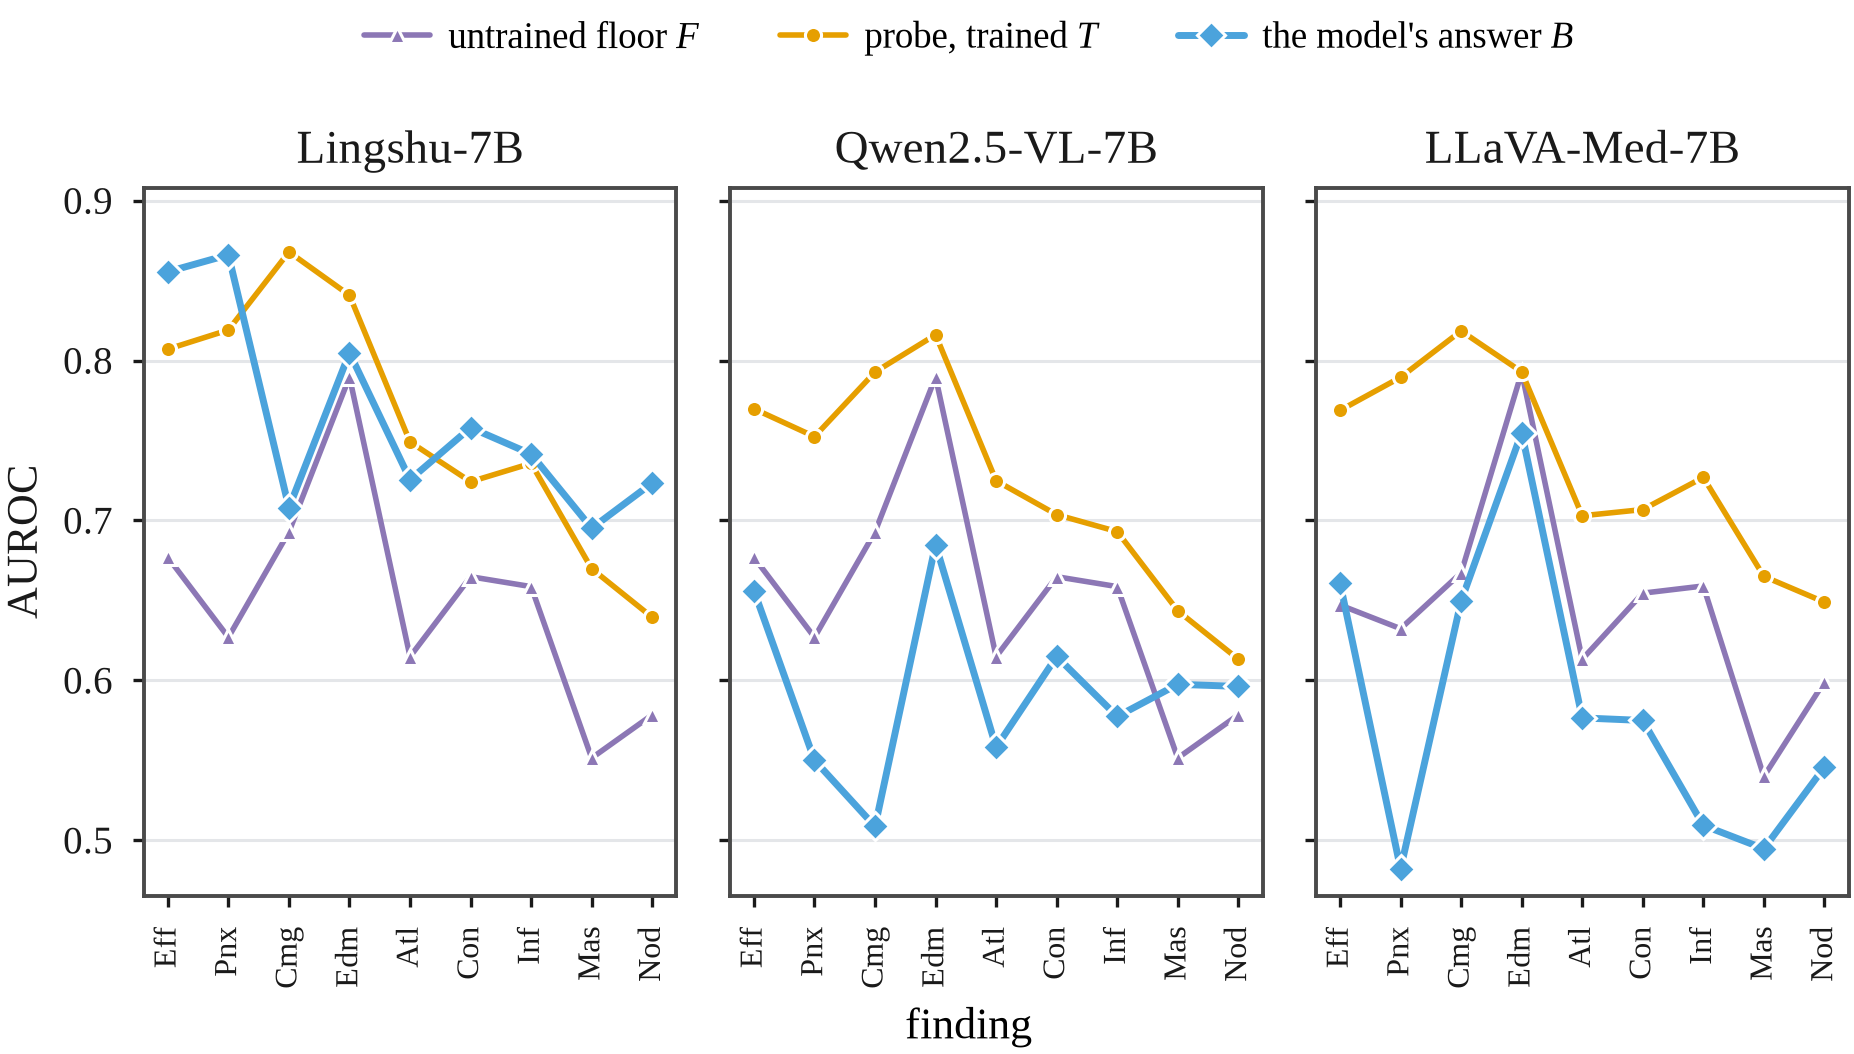
\includegraphics[width=\linewidth]{figures/fig_profile.png}
\caption{\textbf{The same three quantities, finding by finding.} Each panel is one model over the nine
chest-radiograph findings, abbreviated: effusion, pneumothorax, cardiomegaly, edema, atelectasis,
consolidation, infiltration, mass, nodule. $F$ is a probe on an untrained network of the same
architecture, $T$ the probe on the trained model, $B$ the AUROC of the model's own answer. The three
panels are the three cases the paper distinguishes. \textbf{Left}: in Lingshu-7B the answer runs at or
above the trained probe on every finding. \textbf{Centre and right}: in Qwen2.5-VL-7B and LLaVA-Med-7B it
runs below the untrained floor on most of them, while the probe curve is almost the same curve as
Lingshu's. Lingshu-7B and Qwen2.5-VL-7B are the same architecture and share the floor exactly, so the two
left panels differ only in what training did.}
\label{fig:decomp}
\end{figure}

\section{The Second Modality}
\label{app:mod}

\fig{mod} gives the comparison behind the dermoscopy result: for each model, the best AUROC over the
clinical findings against the AUROC of the acquisition variable read from the same features.

\begin{figure}[t]
\centering
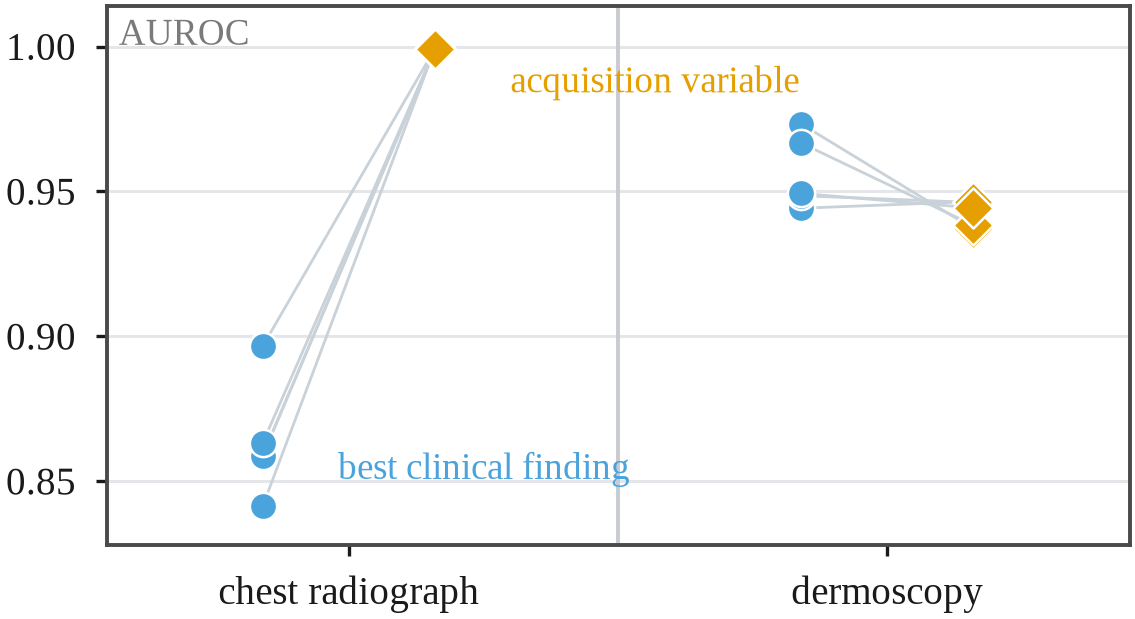
\includegraphics[width=0.62\linewidth]{figures/fig5_modality.png}
\caption{\textbf{Acquisition dominance is a chest-radiograph result.} For each of the five models, the best
AUROC over the clinical findings and the AUROC of the acquisition variable at the same locus set. On chest
radiographs the acquisition variable, view position, outranks every finding in all five models. On
dermoscopy the acquisition variable, anatomic site, outranks the best finding in one of five.}
\label{fig:mod}
\end{figure}

\section{Every Locus, Not Only the One We Report}
\label{app:depth}

\begin{figure}[t]
\centering
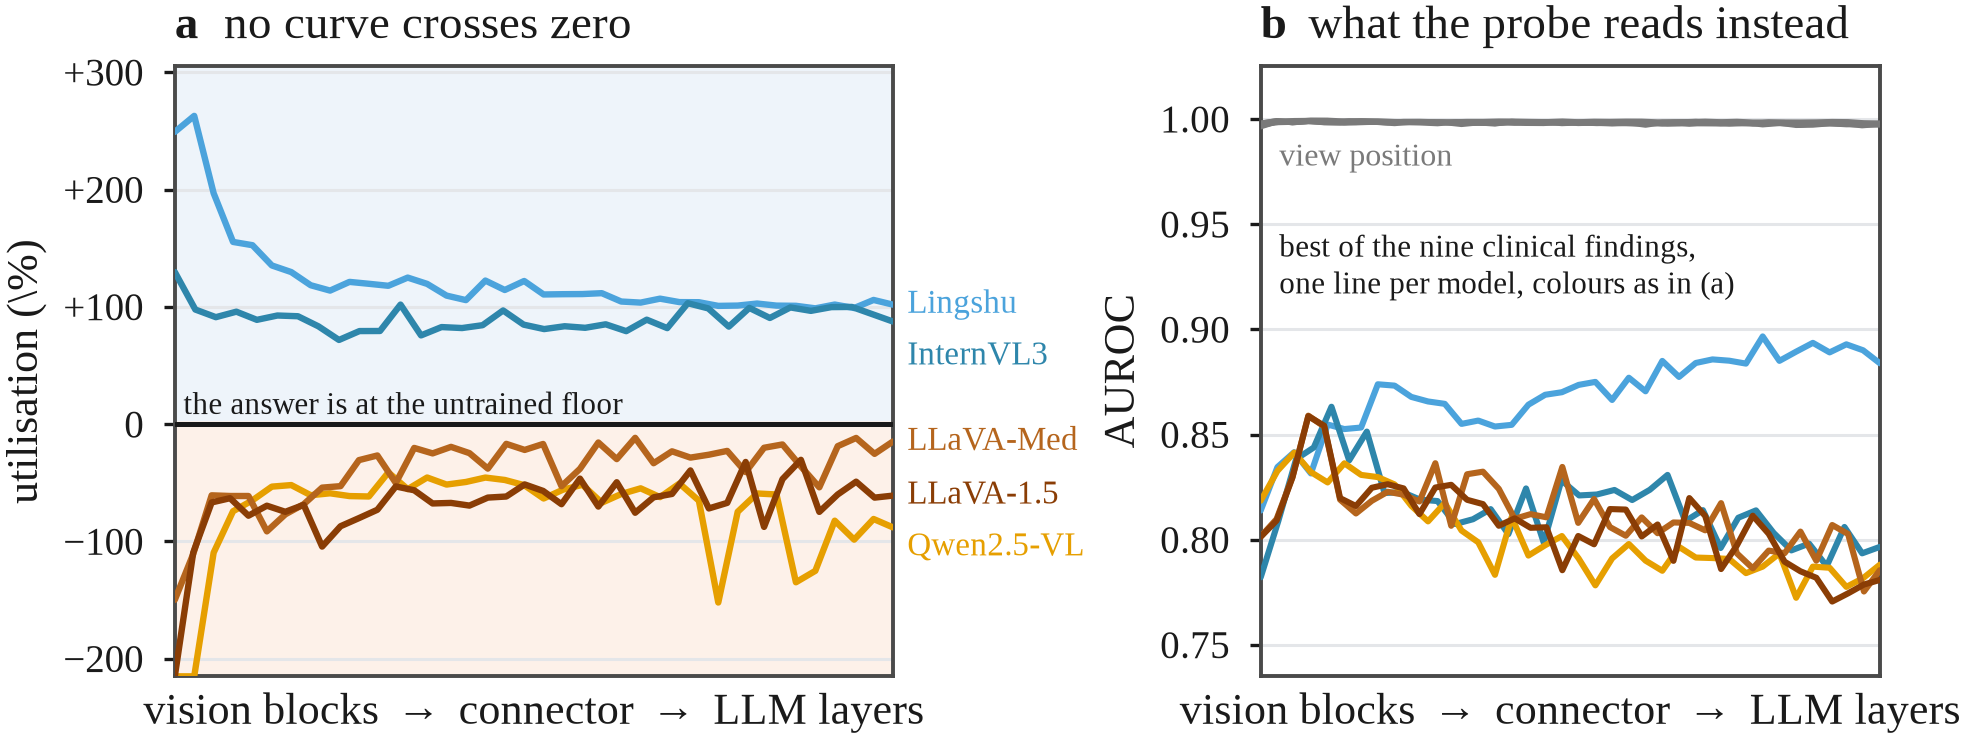
\includegraphics[width=\linewidth]{figures/fig_depth.png}
\caption{\textbf{The conclusion does not depend on which locus we report.} \textbf{(a)}: utilisation at
every prompt-independent locus, from the first vision block through the connector to the last
language-model layer, as the median over the nine findings. Two models sit above zero and three below,
and in 192 model-by-locus points the sign never changes, so reporting any other locus would not have
changed a conclusion. Curves are clipped at the axis limits; Qwen2.5-VL runs to $-565\%$ at four loci.
\textbf{(b)}: what the probe reads instead. View position is decoded above 0.99 at every depth in every
model while the best of the nine findings never reaches 0.90. Colours as in (a).}
\label{fig:depth}
\end{figure}

A probe may be fitted at any of 64 to 72 loci and the best reported, while the model's answer has no such
choice. The fixed connector removes that asymmetry by construction; \fig{depth} shows it also does not
matter, since the sign of utilisation is the same at every prompt-independent locus in every model.

\section{Every Number, Cell by Cell}
\label{app:cells}

The two tables below are generated from the released result files by \texttt{src/make\_tables.py}, so
they cannot drift from the data the way a transcribed number can. Table~\ref{tab:cells} is every cell
behind Figure~\ref{fig:main} and Table~\ref{tab:main}; Table~\ref{tab:elicit} is every cell behind
\fig{controls}.

% generated by src/make_tables.py -- do not edit
\begin{table}[t]
\centering
\small
\setlength{\tabcolsep}{5pt}
\caption{\textbf{Every cell behind Figure~\ref{fig:main}.} $F$ is the probe on the untrained network of the same architecture, $T$ the probe on the trained model, $B$ the AUROC of the model's own answer, and $U=(B-F)/(T-F)$, all at the connector on the same 1000 held-out radiographs. Dashes mark the two cells where $T \le F$, for which the ratio is undefined.}
\label{tab:cells}
\begin{tabular}{@{}ll@{\hskip 8pt}rrrr@{}}
\toprule
Model & Finding & $F$ & $T$ & $B$ & $U$ \\
\midrule
Lingshu-7B & Effusion & 0.677 & 0.807 & 0.856 & $+137$\% \\
 & Pneumothorax & 0.627 & 0.819 & 0.866 & $+124$\% \\
 & Cardiomegaly & 0.693 & 0.868 & 0.708 & $+9$\% \\
 & Edema & 0.790 & 0.841 & 0.805 & $+29$\% \\
 & Atelectasis & 0.615 & 0.749 & 0.726 & $+82$\% \\
 & Consolidation & 0.665 & 0.724 & 0.758 & $+157$\% \\
 & Infiltration & 0.659 & 0.736 & 0.742 & $+108$\% \\
 & Mass & 0.551 & 0.670 & 0.695 & $+121$\% \\
 & Nodule & 0.578 & 0.639 & 0.723 & $+238$\% \\
\midrule
InternVL3-8B & Effusion & 0.511 & 0.791 & 0.818 & $+109$\% \\
 & Pneumothorax & 0.552 & 0.791 & 0.734 & $+76$\% \\
 & Cardiomegaly & 0.552 & 0.822 & 0.621 & $+26$\% \\
 & Edema & 0.666 & 0.811 & 0.787 & $+83$\% \\
 & Atelectasis & 0.530 & 0.722 & 0.659 & $+67$\% \\
 & Consolidation & 0.597 & 0.706 & 0.743 & $+134$\% \\
 & Infiltration & 0.602 & 0.714 & 0.717 & $+102$\% \\
 & Mass & 0.500 & 0.662 & 0.680 & $+111$\% \\
 & Nodule & 0.515 & 0.645 & 0.541 & $+20$\% \\
\midrule
Qwen2.5-VL-7B & Effusion & 0.677 & 0.770 & 0.656 & $-22$\% \\
 & Pneumothorax & 0.627 & 0.752 & 0.550 & $-61$\% \\
 & Cardiomegaly & 0.693 & 0.793 & 0.509 & $-184$\% \\
 & Edema & 0.790 & 0.816 & 0.685 & $-397$\% \\
 & Atelectasis & 0.615 & 0.725 & 0.558 & $-52$\% \\
 & Consolidation & 0.665 & 0.704 & 0.615 & $-129$\% \\
 & Infiltration & 0.659 & 0.693 & 0.577 & $-236$\% \\
 & Mass & 0.551 & 0.643 & 0.598 & $+50$\% \\
 & Nodule & 0.578 & 0.613 & 0.596 & $+51$\% \\
\midrule
LLaVA-Med-7B & Effusion & 0.647 & 0.769 & 0.661 & $+11$\% \\
 & Pneumothorax & 0.632 & 0.789 & 0.482 & $-96$\% \\
 & Cardiomegaly & 0.667 & 0.819 & 0.650 & $-12$\% \\
 & Edema & 0.793 & 0.793 & 0.755 & $+nan$\% \\
 & Atelectasis & 0.613 & 0.703 & 0.577 & $-41$\% \\
 & Consolidation & 0.654 & 0.707 & 0.575 & $-152$\% \\
 & Infiltration & 0.659 & 0.727 & 0.509 & $-221$\% \\
 & Mass & 0.540 & 0.665 & 0.495 & $-36$\% \\
 & Nodule & 0.599 & 0.649 & 0.546 & $-107$\% \\
\midrule
LLaVA-1.5-7B & Effusion & 0.647 & 0.774 & 0.527 & $-94$\% \\
 & Pneumothorax & 0.632 & 0.793 & 0.563 & $-43$\% \\
 & Cardiomegaly & 0.667 & 0.825 & 0.675 & $+5$\% \\
 & Edema & 0.793 & 0.800 & 0.572 & $+nan$\% \\
 & Atelectasis & 0.613 & 0.714 & 0.473 & $-138$\% \\
 & Consolidation & 0.654 & 0.715 & 0.469 & $-307$\% \\
 & Infiltration & 0.659 & 0.716 & 0.539 & $-212$\% \\
 & Mass & 0.540 & 0.669 & 0.575 & $+27$\% \\
 & Nodule & 0.599 & 0.651 & 0.578 & $-40$\% \\
\bottomrule
\end{tabular}
\end{table}

\begin{table}[t]
\centering
\small
\setlength{\tabcolsep}{5pt}
\caption{\textbf{Every cell behind Figure~\ref{fig:controls}.} AUROC of the model's answer under each of the four readouts, the probe at the connector for comparison, and the fraction of the probe-minus-answer gap that the best readout closes.}
\label{tab:elicit}
\begin{tabular}{@{}llrrrr@{\hskip 8pt}rr@{}}
\toprule
Model & Finding & orig. & rephr. & stmt. & neg. & probe & closed \\
\midrule
InternVL3 & Cardiomegaly & 0.595 & 0.621 & 0.541 & 0.585 & 0.822 & 10\% \\
 & Edema & 0.784 & 0.787 & 0.436 & 0.779 & 0.811 & 8\% \\
 & Effusion & 0.814 & 0.818 & 0.803 & 0.809 & 0.791 & --- \\
 & Pneumothorax & 0.658 & 0.606 & 0.525 & 0.734 & 0.791 & 51\% \\
Lingshu & Cardiomegaly & 0.708 & 0.698 & 0.657 & 0.686 & 0.868 & 0\% \\
 & Edema & 0.805 & 0.803 & 0.788 & 0.797 & 0.841 & 0\% \\
 & Effusion & 0.856 & 0.854 & 0.840 & 0.851 & 0.807 & --- \\
 & Pneumothorax & 0.866 & 0.852 & 0.848 & 0.858 & 0.819 & --- \\
LLaVA-1.5 & Cardiomegaly & 0.648 & 0.619 & 0.675 & 0.630 & 0.825 & 13\% \\
 & Edema & 0.532 & 0.564 & 0.485 & 0.572 & 0.800 & 13\% \\
 & Effusion & 0.498 & 0.441 & 0.489 & 0.527 & 0.774 & 9\% \\
 & Pneumothorax & 0.520 & 0.542 & 0.500 & 0.563 & 0.793 & 15\% \\
LLaVA-Med & Cardiomegaly & 0.650 & 0.589 & 0.544 & 0.611 & 0.819 & 0\% \\
 & Edema & 0.755 & 0.650 & 0.601 & 0.716 & 0.793 & 0\% \\
 & Effusion & 0.661 & 0.627 & 0.601 & 0.653 & 0.769 & 0\% \\
 & Pneumothorax & 0.479 & 0.432 & 0.482 & 0.461 & 0.789 & 1\% \\
Qwen2.5-VL & Cardiomegaly & 0.482 & 0.492 & 0.509 & 0.494 & 0.793 & 7\% \\
 & Edema & 0.676 & 0.657 & 0.664 & 0.685 & 0.816 & 5\% \\
 & Effusion & 0.645 & 0.624 & 0.614 & 0.656 & 0.770 & 7\% \\
 & Pneumothorax & 0.529 & 0.520 & 0.497 & 0.550 & 0.752 & 7\% \\
\bottomrule
\end{tabular}
\end{table}


\section{How Each Figure Was Made}
\label{app:figs}

Every figure is produced by a script in the release, from the released result tables, with no manual step.
Each entry names the script, the table it reads and the choices that are not visible in the figure.

\textbf{Figure~\ref{fig:teaser}} (\texttt{src/fig\_teaser.py}, from \texttt{utilisation\_final.csv} and
the per-image score archives). Panel (b) plots the median over the nine findings; panel (c) uses effusion,
the finding for which answer-position activations were cached.

\textbf{Table~\ref{tab:main}} (\texttt{src/utilisation.py}, writing \texttt{utilisation\_final.csv}).
Every entry is the median over the nine findings at the connector. The interval in the last row is the
median over models of the median over findings of the per-estimate 95\% bootstrap width, halved.

\textbf{Figure~\ref{fig:main}} (\texttt{src/fig\_heat.py}, from \texttt{utilisation\_final.csv}). The
diverging scale is pinned to white at zero and clipped at $\pm150\%$; the two Edema cells are blank
because $T \le F$ there, which the ratio cannot express. Cell text is white where the cell is dark enough
to carry it, black otherwise.

\textbf{Figure~\ref{fig:floor}} (\texttt{src/fig\_floor.py}, from \texttt{utilisation\_final.csv}). The
three architectures are the three distinct untrained networks: Lingshu and Qwen2.5-VL share one, LLaVA-Med
and LLaVA-1.5 share another, InternVL3 is the third. The null in panel (c) is 20{,}000 independent random
rankings of the nine findings, one per architecture, with the same statistic recomputed each time.

\textbf{Figure~\ref{fig:dir}} (\texttt{src/fig\_direction.py}, from \texttt{plant\_alignment.csv},
\texttt{plant\_gate.csv} and \texttt{cad\_summary\_v1.csv}). Panel (a) is restricted to the nine cells that
pass the dose-response gate; bands are $\pm1.96$ standard errors of the mean over cells and loci at that
dose. Panel (b) drops cells where either effect is zero, which the log axes cannot show.

\textbf{Figure~\ref{fig:controls}} (\texttt{src/fig\_elicit.py}, from \texttt{elicitation\_summary.csv}).
Rows are sorted by the gap under the original question. Panel (b) shows every cell for every readout, not
only the winner.

\textbf{Figure~\ref{fig:depth}} (\texttt{src/fig\_depth.py}, from the per-locus probe sweeps of both the
trained and the untrained networks). Answer-position loci are excluded throughout, since they depend on
the question that was cached. Curves are medians over the nine findings, clipped at the axis limits.

\textbf{Every figure is checked mechanically before it is written.} \texttt{src/figcheck.py} fails a
figure whose labels overlap each other or the plotted data, whose text leaves its axes, whose legend
covers a series, or whose tick labels are closer than 1.5\,pt. \texttt{src/verify\_draft.py} recomputes
every number quoted in the text and in the captions from the released tables.

\section{The Probe Direction, in Full}
\label{app:dir}

\begin{figure}[t]
\centering
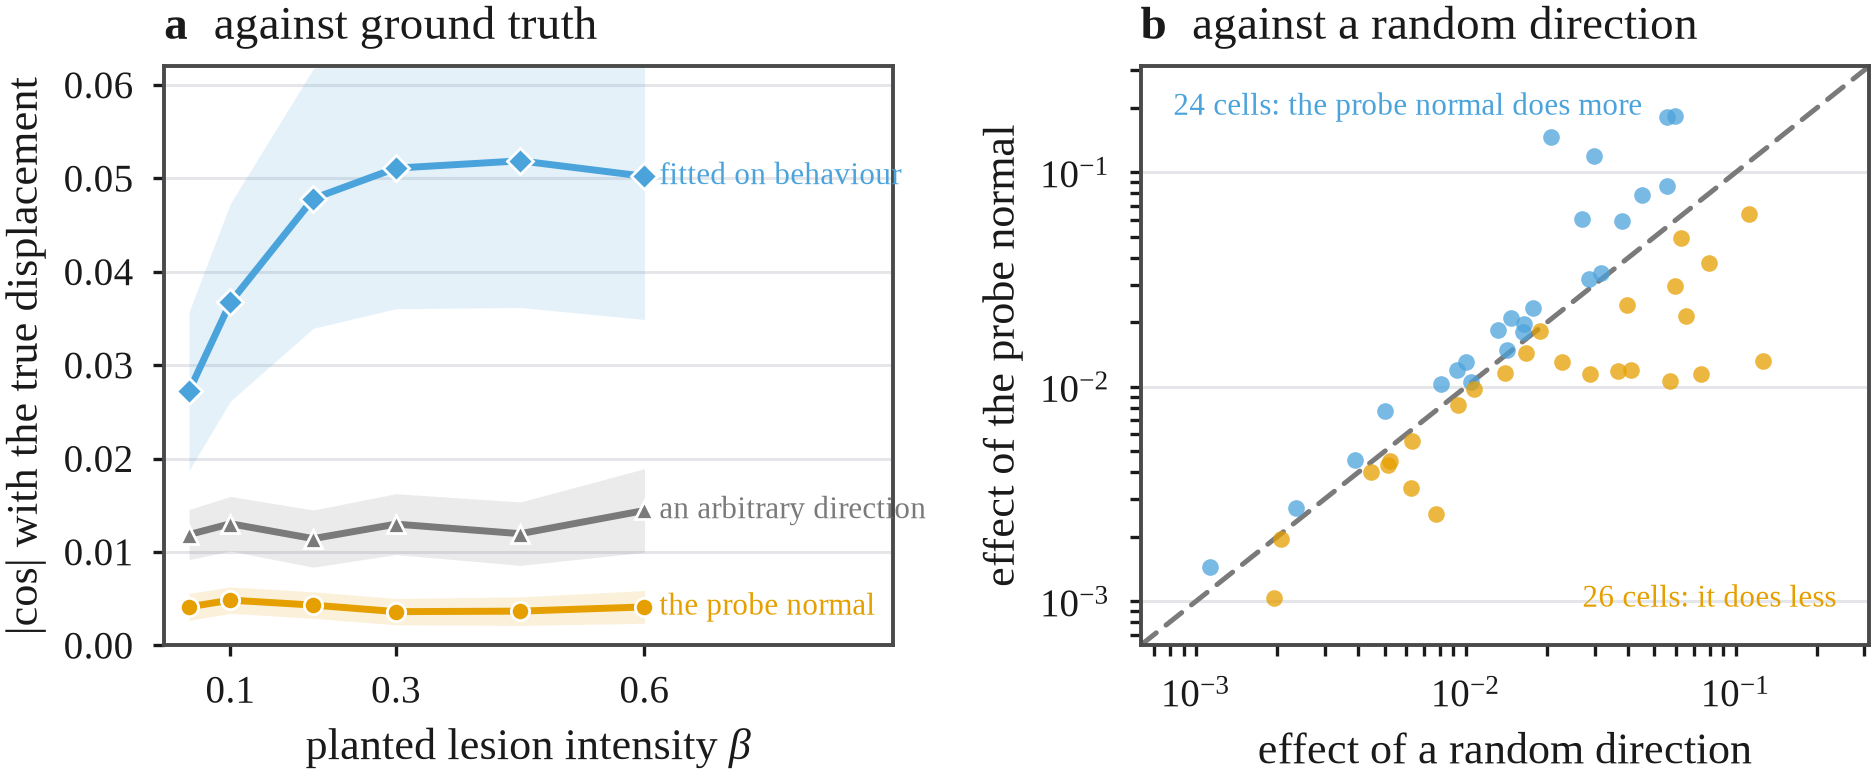
\includegraphics[width=\linewidth]{figures/fig_direction.png}
\caption{\textbf{The probe normal is not the direction the representation uses.} \textbf{(a)}: against
ground truth. A lesion of known intensity $\beta$ is planted and the displacement it causes is recorded,
over the nine cells that pass the dose-response gate. A direction fitted on behaviour climbs with the
dose and plateaus; an arbitrary direction is flat at $0.013$; the probe normal is flat at $0.004$, below
the arbitrary one at every dose. Bands are $\pm1.96$ standard errors. \textbf{(b)}: against a random
direction. The answer change from adding the probe normal against that from a random direction of the
same norm at the same locus and magnitude, one point per model, finding and locus, on log axes with the
identity line. The cloud straddles it, 24 cells against 26.}
\label{fig:dir}
\end{figure}

Panel (a) is the only measurement in the paper with ground truth to be right about, since the displacement
a planted lesion causes is known by construction. Panel (b) is the intervention comparison at every locus
and magnitude in the sweep.

\section{Elicitation in Full}
\label{app:elicit}

\begin{figure}[t]
\centering
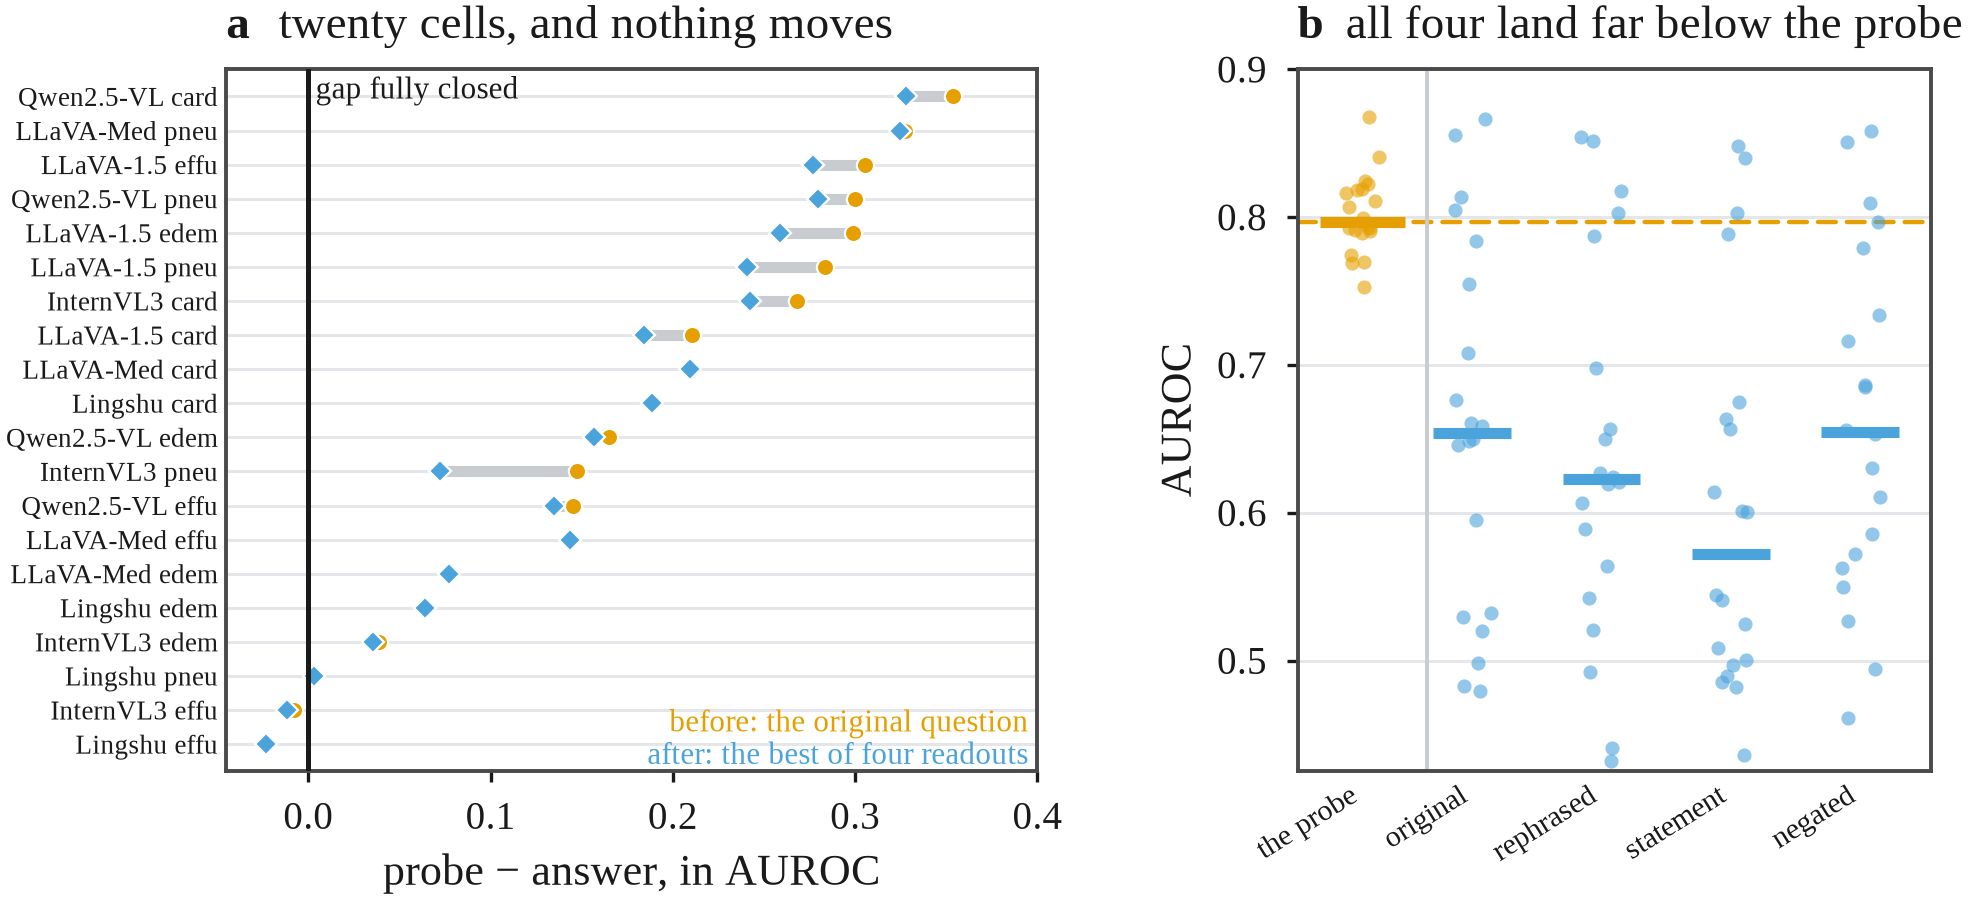
\includegraphics[width=\linewidth]{figures/fig_elicit.png}
\caption{\textbf{Four ways of asking, and the gap does not move.} \textbf{(a)}: one row per
model-by-finding cell, sorted. The circle is the probe-minus-answer gap under the original question, the
diamond is what the best of four readouts leaves, and the bar between them is what elicitation bought.
The median cell closes 7\% of its gap; one of twenty closes more than a fifth. \textbf{(b)}: where each
readout lands. The probe is tight around 0.80 and all four readouts sit far below it with a wide spread,
and which wins is near-uniform over the twenty cells (7, 3, 3, 7), so the winner is a draw among noisy
estimates rather than a method that works.}
\label{fig:controls}
\end{figure}

The four readouts are the original yes-or-no question, an alternate phrasing of it, the log-probability of
the complete statement against its negation, and a negation-symmetrised score. \fig{controls} shows both
what each bought and where each landed.

\section{The Validity Battery in Full}
\label{app:battery}

A probe score without controls is not interpretable, and the survey that motivated this work found the
relevant controls almost entirely absent. Every probe number reported here carries four.

\textbf{A permutation null.} Labels are permuted within the training split and the probe refitted, giving
the chance floor for that fit at that locus rather than an assumed 0.5.

\textbf{A randomised control task} \citep{hewitt2019designing}. Each input \emph{type} receives a fixed
random label, and selectivity is the real AUROC minus the control AUROC. A control task needs many types:
with two types the random assignment is one of four functions, two constant and two equal to the type
itself, so the control merely asks whether the type is decodable. Measured on Qwen2.5-VL, view position
decodes at 0.999 at every locus, which drove a two-type control to 0.999 and selectivity negative. The
type used here is therefore the cross of the acquisition variable, sex and age decade, giving 39 types on
radiographs and 67 on dermoscopy, all of which recur on both sides of a patient-level split. This is not a
strict Hewitt and Liang control task, because images have no equivalent of word identity, and we say so
rather than imply otherwise.

\textbf{Nuisance probes.} The acquisition variable and sex are decoded at the same locus from the same
features, so that a finding probe which is really reading acquisition can be seen to be doing so.

\textbf{The untrained floor}, which Section~\ref{sec:test3} shows is the only one of the four that
separates what a model learned from what its input statistics provide.

\section{What Depends on the Prompt, and What Does Not}
\label{app:prompt}

Activations were cached under one finding's question. Whether that matters is measurable rather than
assumable, so we measured it: changing the question changes the answer-position activations by 6\% to 34\%
in relative norm and changes the visual-position, connector and vision-tower activations by exactly
$0.000000$. The reason is structural. Visual tokens precede the question text in the sequence and
attention is causal, so no information from the question can reach a visual position. Answer-position loci
are consequently valid only for the finding whose question was cached, and are excluded elsewhere. Every
number in this paper comes from a prompt-independent locus.



\section{Score Distributions for All Five Models}
\label{app:dist}

AUROC summarises a ranking and can hide the shape that produced it. \fig{dist} shows the two score
distributions themselves, which is where the extreme case is visible as a shape rather than as a number.

\begin{figure}[t]
\centering
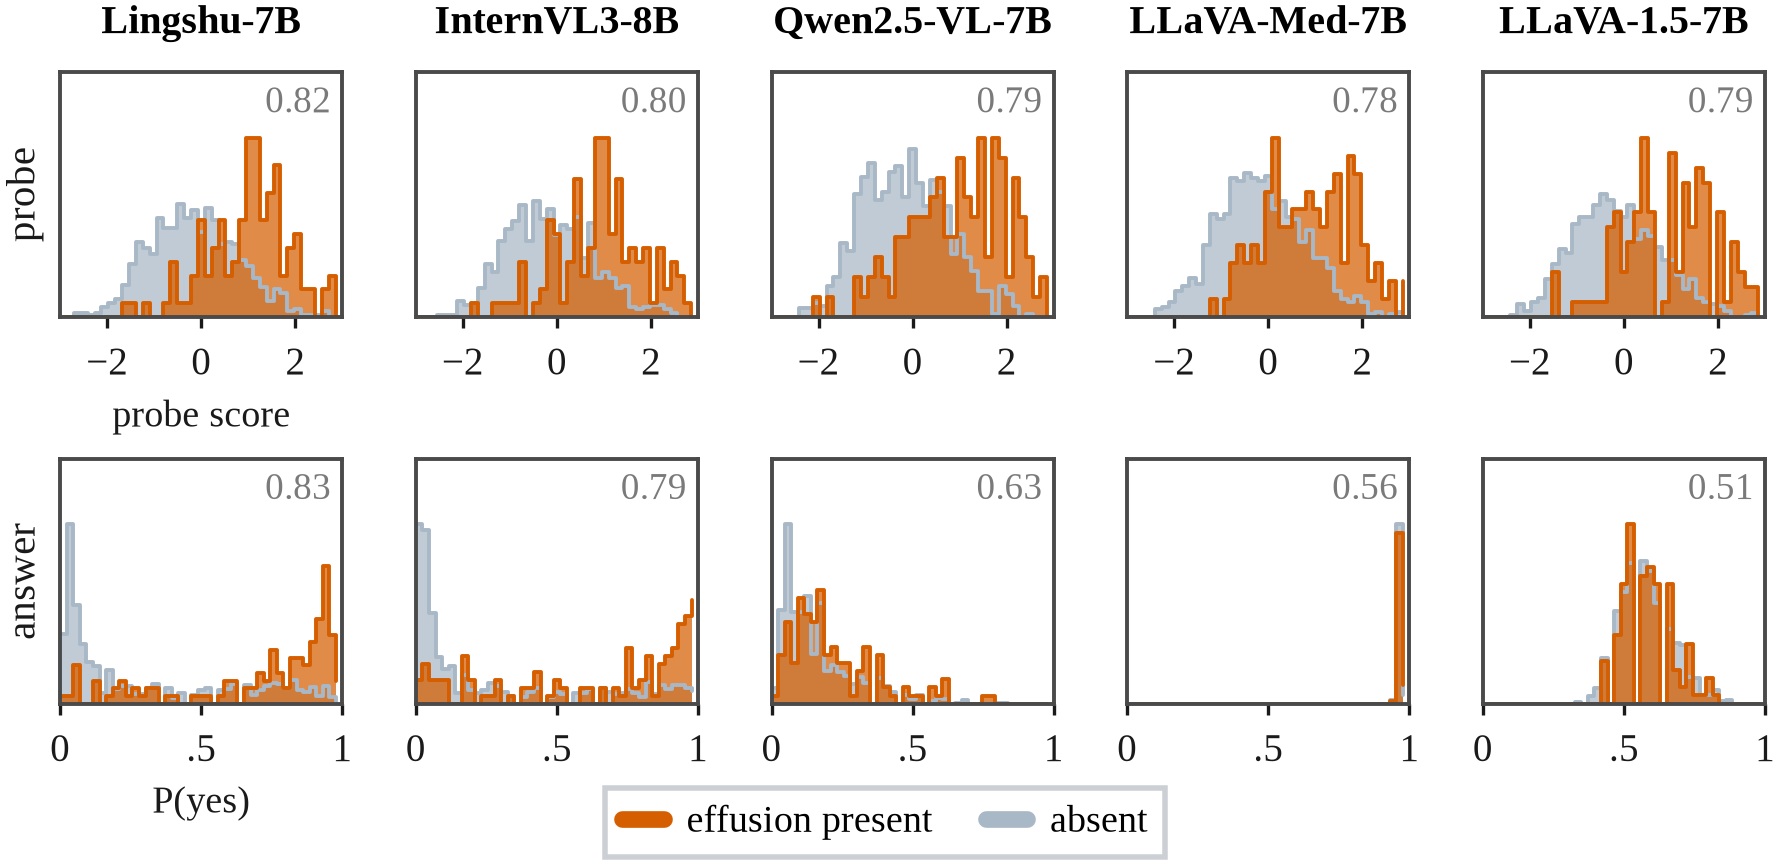
\includegraphics[width=\linewidth]{figures/fig0_distributions.png}
\caption{\textbf{The probe rows are near-copies of one another. The answer rows are not.} The two scores
of \fig{teaser}a, for all five models and the effusion question, on the same 1000 held-out radiographs.
\textbf{Top}: the probe's decision value, standardised within each model. \textbf{Bottom}: the model's own
$P(\mathrm{yes})$. The number in each panel is that panel's AUROC.}
\label{fig:dist}
\end{figure}

\section{Implications in Full}
\label{app:impl}

\subsection*{For anyone reporting a probe score}

Report three numbers rather than one: the probe score, the same probe on an untrained network of the same
architecture, and the model's own behavioural score on the same rows. Their combination is utilisation,
and it answers the question a probe score is usually taken to answer. The cost is one extra extraction
pass and one extra forward pass per image and finding, against a seventy-locus probe sweep these studies
already run. What it buys is the difference between a fact about the model and a fact about the images: on
oedema an untrained network reaches 0.793 and training adds 0.039, so 95\% of what a probing study would
report for that finding is available before the model has seen a radiograph. A floor also changes what a
null result means, since a finding read at 0.62 over a floor of 0.54 received more from training than
oedema did.

\subsection*{For anyone comparing models with a probe}

Do not. The two orderings disagree. Probing places Lingshu-7B and LLaVA-Med-7B within 0.02 of each other;
their answers differ by 0.19 and their utilisations by 189 points. A study that selected a model on probe
scores would have been indifferent between the best and the worst model in our set.

The failure is not that probing is noisy. The scores are stable, reproduce across loci and carry proper
controls; they measure something real that is not the quantity a model comparison needs. This bears
directly on the interpretability literature on medical models, which reports probe curves across depth for
several models at once and reads the differences between them as differences in what the models learned.
Those differences are within the range over which, in our data, behaviour varies by a factor of five.

\subsection*{For anyone building a medical vision-language model}

Three of our five models carry clinically decodable information their answers do not reach. On LLaVA-Med
the answer sits below the untrained floor on eight of nine findings while a probe reads those same
findings from its activations at 0.65 to 0.86. The gap is an offer as much as a diagnosis: a linear head
on an existing representation is a few hundred parameters and needs no retraining of the backbone.

It is also a warning about evaluation. A model that answers yes to every finding on every radiograph will
pass any evaluation that asks whether the information is present and will fail a clinician immediately,
and no probing evaluation we are aware of would surface that.

Finally, the matched pairs say that ``medical pretraining'' is not the operative variable. Lingshu-7B and
Qwen2.5-VL-7B share an architecture and a floor and differ by 183 points of utilisation, but LLaVA-Med-7B
and LLaVA-1.5-7B, also a medical and general pair, differ by half a point. Whatever produced Lingshu's
utilisation is a property of how it was trained and not of the fact that it was trained on medical data.
Identifying it is the obvious next question and five models cannot answer it.

\subsection*{What this does not show}

It does not show that these representations are unused for anything. It shows that one output pathway, a
yes-or-no answer to a direct question, does not reach most of what training added. A different head, a
different prompt format, or a fine-tuned readout might, and the previous subsection is an argument that
one of them should.

\subsection*{For anyone deploying one}

A model's answer is the only thing a clinician sees. Two of our five models answer as well as any linear
readout of their own activations; three answer worse than a probe on a network that was never trained.
Nothing about a model's probe scores, its parameter count, or whether it was trained on medical data
predicts which group it falls into, and the only measurement that does predict it is the one a deployment
evaluation would run anyway: score the model's own answers against labels on held-out patients.

The corollary is that a published probe result should not be treated as evidence that a model is safe to
ask. It is evidence that the information is somewhere in the network, which is compatible with the model
answering the same way regardless of what it is shown.

Two of our models make the point in opposite directions. Lingshu-7B answers effusion better than any
linear readout of its own connector, so its representation understates what the system does. LLaVA-Med-7B
answers the same question at 0.56 while a probe reads 0.79 from the same activations, so its
representation overstates it. A deployment decision taken on the probe number would have been wrong about
both, in opposite directions.

Finally, utilisation is cheap enough to compute during model selection rather than after deployment. It
needs a held-out set with labels, which any clinical evaluation already has, one untrained instantiation
of the architecture, which is a configuration file and a random seed, and the model's own answers, which
the evaluation collects anyway. Nothing about it requires access to training data or to the training
recipe.

\section{Design Faults Found and Fixed During This Work}
\label{app:faults}

The paper's argument is that unchecked measurement produces confident errors. Our own measurement was no
exception, and each of the following would have produced a number that looked publishable and was wrong.
Every number quoted in the paper is recomputed from the released result tables by a script that fails if
any quoted value disagrees with the data; it currently checks 52 values.

\begin{table}[h]
\centering
\small
\begin{tabular}{p{0.42\linewidth}p{0.50\linewidth}}
\toprule
Fault & What it would have shown \\
\midrule
Control task over two input types & selectivity of $-0.19$, ``probes are anti-informative'' \\
Perturbation scaled as $\alpha/\sqrt{D}$ & ``no locus is steerable'', from a sweep that never exceeded
13\% of the activation norm \\
Magnitude scaled by the pooled norm but applied per token & cross-locus comparisons confounded with depth,
the ratio running from $0.42\times$ to $1.64\times$ \\
A structurally severed locus left in the steering set & a causally dead locus scored as ``not steerable'' \\
An Adam step of norm 3.0 applied to a unit vector & specificity weights of 3.0 and 0.0 producing identical
runs \\
\texttt{gradient\_checkpointing\_enable()} on a model in \texttt{.eval()} & a silent no-op; three jobs died
of memory while reporting checkpointing was on \\
\texttt{.detach()} inside a checkpointed block & every direction-fitting job dying at the second locus \\
Evaluation images screened by dataset label rather than model baseline & ``this representation is
unsteerable'', for a model with 0.033 of headroom \\
A 1000-row behavioural score joined to a 5343-row probe score & a gap inflated by comparing different
samples \\
All activations cached under one finding's prompt & answer-position probes for the other eight findings
reading the wrong prompt's activations \\
A nuisance analysis reading one of four site indicators & dermoscopy nuisance dominance reported as 0 of 5
rather than 1 of 5 \\
A font package with no bold face & every bold lead-in and every bold caption claim rendering at regular
weight, without an error \\
\bottomrule
\end{tabular}
\end{table}

\section{Claims Retired During This Work}
\label{app:retired}

\textbf{``The peak of decodability is never the peak of steerability, in 15 of 15 cells.''} With $k$ loci
and two independent argmaxes this holds by chance with probability $(1-1/k)^{15}$, which is 0.27 at the 12
loci we steer and 0.81 across all 70 probe loci. It is what the null predicts.

\textbf{``29 intervention effects pass the selectivity test, 14 with inverted sign.''} A
leave-one-random-out audit puts the null pass rate at 8.21\%, or 29.6 expected rows out of 360, against 29
observed.

\textbf{``Causal separability of 1.0 shows no concept-specific direction can exist at the readout.''} The
analysis averaged the magnitude of a \emph{signed} cosine. The per-step sequence at that locus is
$[-1, +1, -1, -1, +1]$, where $+1$ is a conflict and $-1$ a synergy, and averaging magnitudes merged the
two. The value near one there is also an architectural necessity, since the only computation downstream is
a norm and a yes-minus-no readout shared by every question.

\textbf{``The untrained floor is predicted by the label's correlation with view position, $r = +0.65$.''}
Downgraded rather than retired, and reported in Section~\ref{sec:test3} as an association: with nine
findings it is not significant ($p = 0.06$) and removing oedema leaves $r = 0.42$.

\end{document}
